% !TEX root =  paper.tex
\section{Discussion}\label{sec:discussion} 

\begin{figure}[t]
\centering
%\fbox{
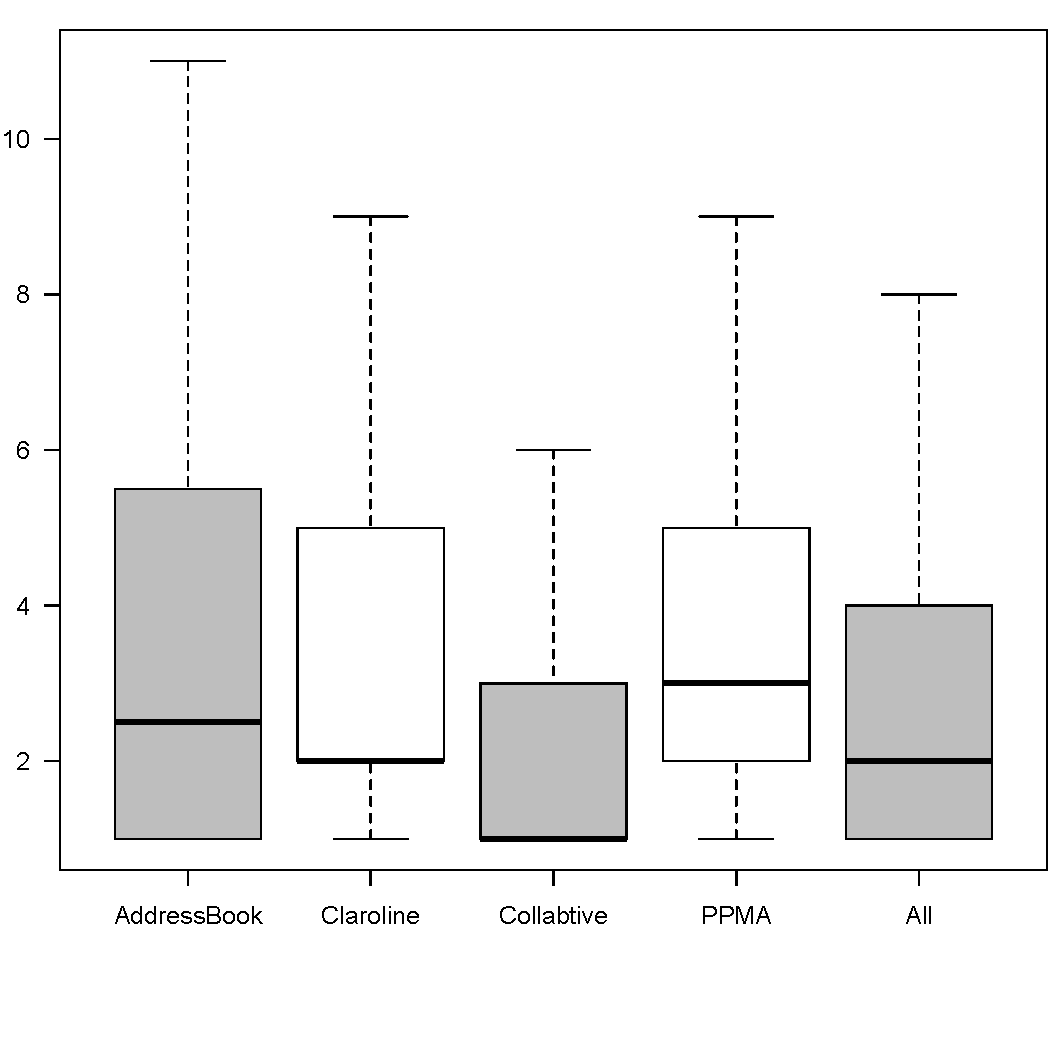
\includegraphics[trim={0cm 0cm 0cm 0cm}, clip,width=0.8\columnwidth]{images/distribution.pdf}
%}
\caption{Distribution of test breakages per test case in each subject system.}
\label{fig:distribution}
\end{figure} 

In this section, we discuss some of our evaluation findings, tool design decisions and limitations, as well as threats to validity of our study.

\head{Prevalence} Our empirical study results confirm that E2E web tests suffer from the fragility problem as the web application evolves. Indeed, 329/2672 tests of our benchmark (12\%) experienced at least one breakage that the test engineer must inspect, and find an appropriate repair for. 
\autoref{fig:distribution} shows box-plots about the distribution of breakages per test cases in each subject system. We observe that most of the tests of the tests have on average between 1--5 breakages per test. 
In short, (1)~test suites tend to break frequently as the web application evolves, and (2)~breakages may pertain occur multiple times within the same test. 

\head{Automatic Repair} 
Our evaluation revealed that \tool can repair more than 80\% of the total number of breakages correctly. Therefore, we believe \tool is accurate in its repair task.

Regarding the efficacy of \tool, we investigated why \emph{all}  breakages were not repaired. We enumerate some of the main reasons next, which pertain to both the inherent nature of our subjects tests and some of our design decisions in developing \tool. 
First, we cannot 
Second, 
Third, 
Fourth, 
Fifth, .  
Sixth, . 
Finally, we do not reorganize flaky (non-deterministic) tests, multithreaded tests, or tests that have read/write dependencies on external resources such as files.

\head{Limitations}
We currently do not support the creation of general purpose statements, such as the ones that need input data.

\head{Performance and Overhead} 
On the whole, we believe that the potential benefits outweigh the foreseeable overhead given (1)~our results in the automated repairs, (2)~the speed of our image processing pipeline. However, should strict time constraints apply, the pre-processing step can be carried out overnight.

Manually inspecting the application to find a candidate repair  and create a locator for the broken statement can be in fact quite time-consuming. Our own experience in repairing tests, which we were required to do while devising \tool, corroborates the costliness of the task. For example, in AddressBook, one of the test for the search functionality fails 11 times when applied from version 4.02 to version 4.1.1: three elements gets removed (Scenario~3) and seven mis-selections occur (Scenario~4). \tool created the visual dynamic execution trace of the test in 22 s, and then it found correct repairs for all 11 breakages in $\approx$57 s. Thus, in this specific case, our technique can have prospect for success if the manual detection and repair performed by a human tester is lower than 80~s. When considering the aggregate results, the overhead imposed by our technique amply justify its adoption, given the benefits as far as automatic repair is concerned.  

\head{Applications} 
\begin{itemize}
\item screenshots can be used to automate software oracles
\item our approach is robust to both shifting and scaling (invariant to translation and scale transformation)
\item runtime detection (monitoring) technique
\item self-repair technique
\item root cause analysis
\end{itemize}

\subsection{Potential for Hybridization} 

\subsection{Threats to Validity}\label{sec:ttv}

\head{Internal validity} We limited the bias of having produced test suites ourselves, that could constitute a threat to the internal validity of our work, by choosing existing test suites used in the previous web testing research. This also ensures, to some extent, that the chosen object of analysis are non-trivial, therefore representative of a test suites that a real web tester would implement. 

\head{External validity} Concerning the generalizability of our results, we ran our approach with a limited number of subjects and test suites. However, we believe the approach to be applicable in a general web testing scenario, even though the magnitude of the results might change when considering different test suites and applications. To limit biases in the manual selection of the versions, we considered \textit{all} the available releases after those for which the test suites were developed for.